% =====================================================================
\chapter{Results and Discussion}
\label{ch:results}
% =====================================================================

This chapter reports what the experiments actually show. We are deliberately strict about
provenance: a number appears here only if a saved measurement file supports it, and we
keep in-distribution detection separate from cross-task transfer at all times. The chapter
first states which experiments are complete and which are still running, then presents the
in-distribution results, then the full transfer results for the one model with a complete
set of measurements, then a partial second model, and finally the discussion.

\section{What has been measured}

The study spans several models, but they are at different stages of completion, and it
would be misleading to present them as a finished sweep. Table~\ref{tab:status} states the
status of each model honestly. One six-billion-parameter model has a complete set of
measurements --- all sixteen configurations and all six baselines, on all ten benchmarks,
scored on identical rows --- and it anchors this chapter. A second model of comparable size
has a verifiable diagnostic run plus an extended run whose consolidated file is not yet
archived. The remaining large models have generated their training data but do not yet
have reported detection results, and are marked accordingly.

\begin{table}[h]
\centering
\caption{Status of each model at the time of writing. Only the model with a complete,
file-backed set of measurements is used for the headline comparison.}
\label{tab:status}
\small
\renewcommand{\arraystretch}{1.2}
\begin{tabular}{l c l}
\toprule
\textbf{Model} & \textbf{Training examples} & \textbf{Status} \\
\midrule
GPT-J (6.0\,B)      & 2000 & complete: 16 configurations + 6 baselines, 10 benchmarks \\
OPT (6.7\,B)        & 2000 & partial: diagnostic run verified; extended run pending archival \\
Qwen2.5 (3\,B)      & 2000 & in-distribution configurations only (no baseline run) \\
TinyLlama (1.1\,B)  & ---  & earlier in-distribution figure only \\
Mistral (7\,B)      & 2000 & data generated; detection results pending \\
Falcon (7\,B)       & 2000 & data generated; detection results pending \\
Llama-2 (7\,B)      & 400  & gated access; undersized data; results pending \\
GPT-2 (0.12\,B)     & 1000 & smoke test; diagnostic only, not a result \\
\bottomrule
\end{tabular}
\end{table}

\section{In-distribution detection}

We begin with the easier regime, in which the detector is tested on held-out text of the
same kind it was trained on. An earlier mid-term evaluation, run on a larger
ten-thousand-sample corpus with the canonical feature alone, reported in-distribution
AUROC of $0.673$ for the three-billion model and $0.592$ for the one-billion model, and
noted that the larger model carried the stronger internal signal. These are encouraging
numbers, but they are in-distribution and were obtained at a larger data scale than the
unified runs reported below.

At the two-thousand-sample scale of the unified pipeline, in-distribution AUROC is more
modest. On the three-billion model the configurations sit between roughly $0.39$ and
$0.47$, and on the six-billion model they sit between roughly $0.40$ and $0.55$. The drop
relative to the mid-term figure is consistent with the smaller training set and the harder,
fully unified evaluation; it is a reminder that sample size matters and that a single
favourable number should not be over-read. Figure~\ref{fig:indist} places the in-distribution
and transfer numbers side by side and makes the central point of this chapter visible at a
glance: in-distribution detection, while imperfect, is clearly easier than transferring to
unseen task types.

\begin{figure}[t]
\centering
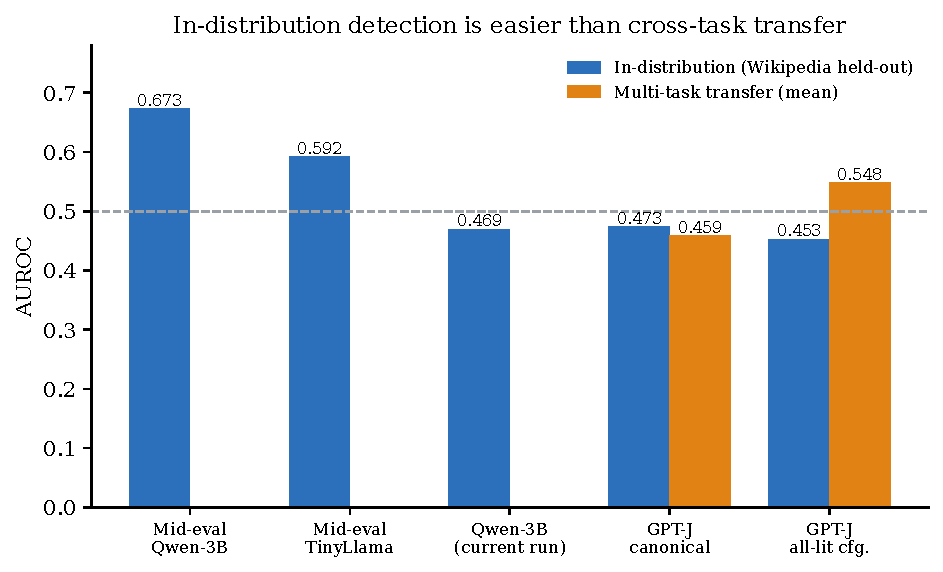
\includegraphics[width=0.84\textwidth]{images/ch05_results/ch05_4_indist_vs_transfer.pdf}
\caption{In-distribution detection is easier than cross-task transfer. The two left bars
are earlier mid-term in-distribution figures at a larger data scale; the rest are from the
unified runs. Transfer means are computed over the ten-benchmark suite.}
\label{fig:indist}
\end{figure}

\section{Transfer results on the fully measured model}
\label{sec:gptj}

We now turn to the substantive result: cross-task transfer on the six-billion-parameter
model, for which every configuration and baseline was measured on the same rows of all ten
benchmarks. Table~\ref{tab:gptj-configs} reports the sixteen configurations and
Table~\ref{tab:gptj-base} the six baselines, each by mean transfer AUROC; the full
per-benchmark matrix is given in Appendix~\ref{app:tables}.

\begin{table}[h]
\centering
\caption{Six-billion-parameter model: the sixteen feature configurations, by mean transfer
AUROC over ten benchmarks, with the in-distribution figure for reference. Higher is
better; $0.5$ is chance.}
\label{tab:gptj-configs}
\small
\renewcommand{\arraystretch}{1.15}
\begin{tabular}{cl c c}
\toprule
\textbf{Cfg.} & \textbf{Feature content} & \textbf{In-distribution} & \textbf{Mean transfer} \\
\midrule
C1  & Canonical feature only                       & 0.473 & 0.459 \\
C2  & + drift                                      & 0.500 & 0.447 \\
C3  & + cross-layer variance                       & 0.525 & 0.445 \\
C4  & + predictive entropy                         & 0.404 & 0.472 \\
C5  & + internal-state trio (\emph{this work})     & 0.500 & 0.464 \\
C6  & + lookback ratio                             & 0.524 & 0.445 \\
C7  & + logit-lens divergence                      & 0.498 & 0.446 \\
C8  & + confidence margin                          & 0.546 & 0.476 \\
C9  & + lookback/lens/margin trio                  & 0.481 & 0.446 \\
C10 & + all nine literature features               & 0.453 & \textbf{0.548} \\
C11 & + internal-state trio + lookback/lens/margin & 0.540 & 0.525 \\
C12 & + internal-state trio + all literature       & 0.475 & 0.468 \\
C13 & + vocab projection + curvature               & 0.488 & 0.451 \\
C14 & + confidence-trajectory/rank/echo            & 0.405 & 0.546 \\
C15 & + vocab projection/curvature/confidence      & 0.508 & 0.471 \\
C16 & + internal-state trio + all exploratory      & 0.507 & 0.508 \\
\bottomrule
\end{tabular}
\end{table}

\begin{table}[h]
\centering
\caption{Six-billion-parameter model: the six baselines, by mean transfer AUROC over ten
benchmarks. The strongest method overall is the supervised mid-layer probe.}
\label{tab:gptj-base}
\small
\renewcommand{\arraystretch}{1.2}
\begin{tabular}{l c c}
\toprule
\textbf{Baseline} & \textbf{In-distribution} & \textbf{Mean transfer} \\
\midrule
SAPLMA (mid-layer probe)   & 0.419 & \textbf{0.562} \\
Perplexity (mean NLL)      & ---   & 0.523 \\
HalluShift                 & 0.519 & 0.509 \\
HaloScope                  & 0.506 & 0.508 \\
MIND (final-layer probe)   & ---   & 0.487 \\
EigenScore                 & 0.515 & 0.487 \\
\bottomrule
\end{tabular}
\end{table}

The picture that emerges is mixed, and we report it as such. Ranked by mean transfer
AUROC, the strongest method is the supervised mid-layer probe, SAPLMA, at $0.562$. The two
best feature configurations follow closely: the all-literature configuration at $0.548$
and the confidence-trajectory configuration at $0.546$, with the configuration that adds
the internal-state trio to a small literature subset close behind at $0.525$. The simple
perplexity reference scores $0.523$, ahead of the more elaborate HalluShift, HaloScope,
final-layer MIND, and EigenScore baselines, all of which sit between $0.487$ and $0.509$.
Figure~\ref{fig:configs} and Figure~\ref{fig:methods} show these comparisons graphically.

\begin{figure}[t]
\centering
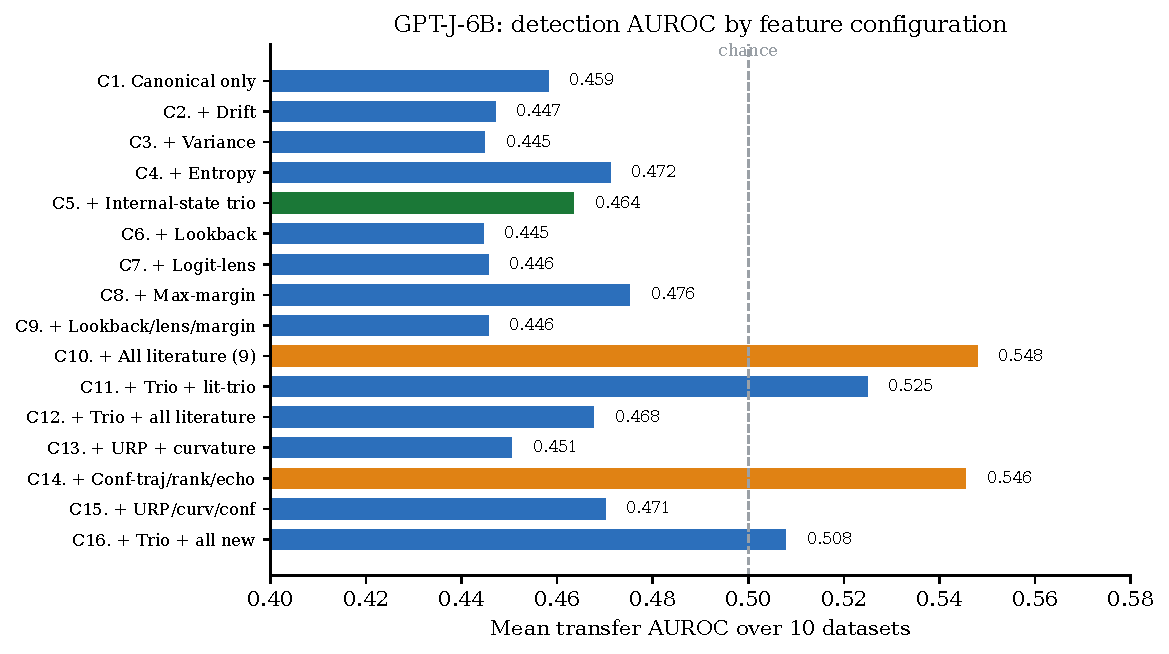
\includegraphics[width=0.95\textwidth]{images/ch05_results/ch05_1_gptj_config_auroc.pdf}
\caption{Mean transfer AUROC of the sixteen configurations on the six-billion model. The
three-feature internal-state set (highlighted) gives only a small change over the
canonical backbone; the gains come from the richer stacks (highlighted).}
\label{fig:configs}
\end{figure}

\begin{figure}[t]
\centering
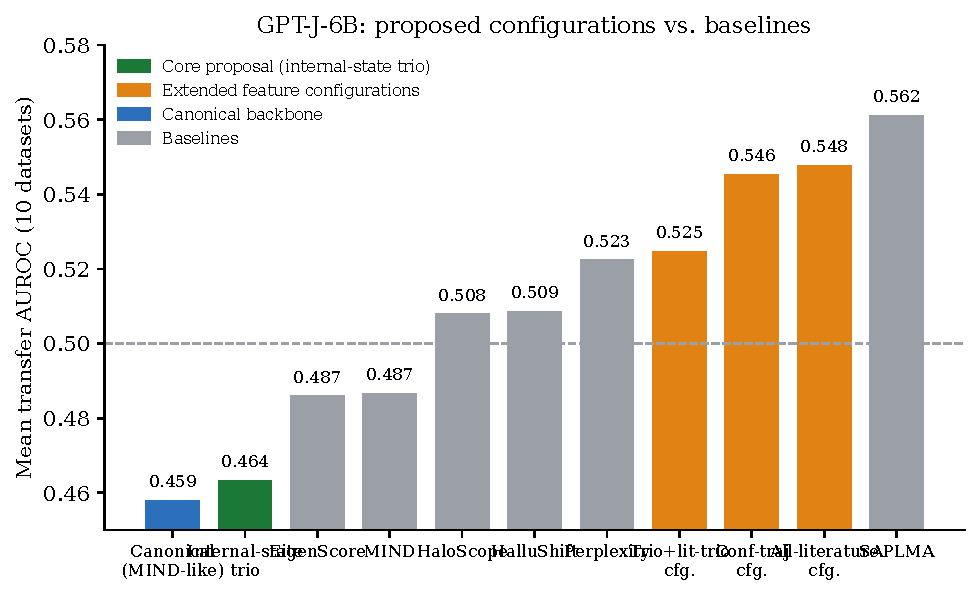
\includegraphics[width=0.95\textwidth]{images/ch05_results/ch05_2_gptj_method_vs_baselines.pdf}
\caption{The proposed configurations against the baselines on the six-billion model. The
best configurations are competitive with the field but do not overtake the strongest
baseline, the supervised mid-layer probe.}
\label{fig:methods}
\end{figure}

Three observations follow directly from these numbers. First, the three core
internal-state features, taken alone on top of the canonical feature (configuration~5),
move the mean transfer AUROC only slightly, from $0.459$ to $0.464$; the individual
additions are mixed, with predictive entropy and the confidence margin helping a little
and drift or variance alone not helping. The lift that does appear comes from the richer
combinations of many features at once. Second, the strongest baseline reads a
\emph{mid-network} layer, while the canonical feature and the MIND baseline read the
\emph{final} layer, and the mid-layer probe is clearly better here ($0.562$ versus
$0.487$). This echoes the layer-selection problem flagged in the literature: on this
model the last layer is not the most informative place to look. Third, none of the
methods is far above chance on transfer; the averages sit in the high-$0.4$ to
mid-$0.5$ range, which is honest evidence that transferring an encyclopedia-trained probe
to unseen task types is hard.

\section{One benchmark dominates the averages}

Before reading too much into the rankings, it is important to see how they are formed.
Figure~\ref{fig:heatmap} shows the per-benchmark AUROC for a representative set of methods,
and Figure~\ref{fig:dominance} traces the same numbers as lines. One benchmark, the
question-answering subset of HaluEval, behaves very differently from the rest: the
mid-layer probe reaches $0.985$ on it, the confidence-trajectory configuration $0.94$, and
the all-literature configuration $0.84$, while on the other nine benchmarks almost every
method hovers near $0.5$. Because this one column is so high, it pulls the averages up and
largely determines the ranking. The honest reading is that the headline averages are
carried by a single, unusually separable benchmark, and that on the remaining benchmarks
the methods are much closer together and much closer to chance. A ranking that looks
decisive on paper is, on inspection, the product of one easy column.

\begin{figure}[t]
\centering
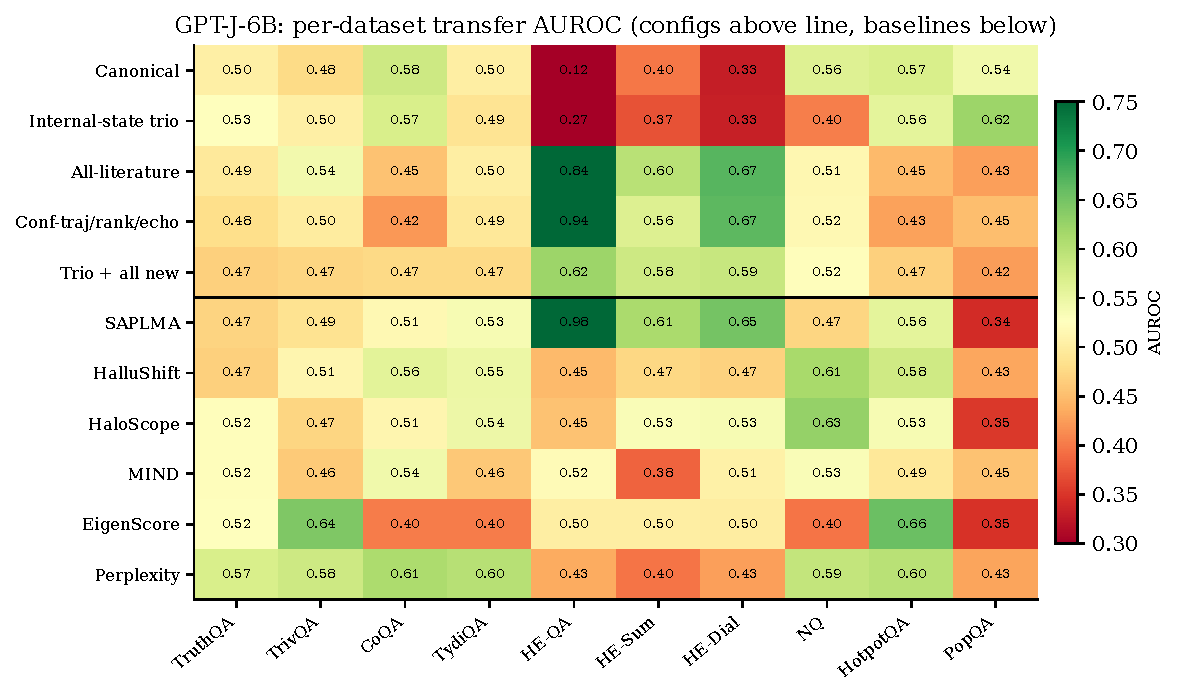
\includegraphics[width=0.99\textwidth]{images/ch05_results/ch05_3_gptj_heatmap.pdf}
\caption{Per-benchmark transfer AUROC on the six-billion model, configurations above the
line and baselines below. The HaluEval-QA column stands out; elsewhere most cells are near
$0.5$.}
\label{fig:heatmap}
\end{figure}

\begin{figure}[t]
\centering
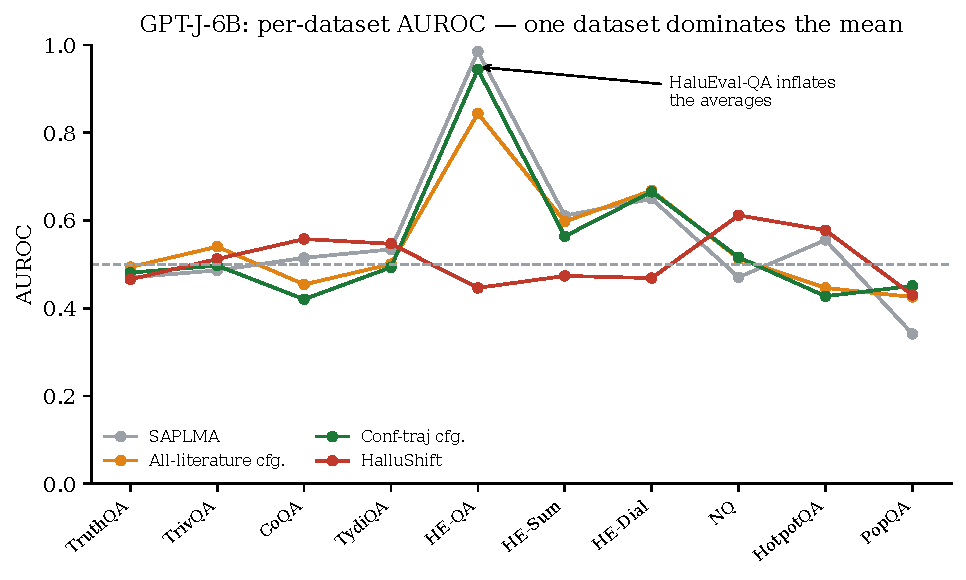
\includegraphics[width=0.86\textwidth]{images/ch05_results/ch05_5_halueval_dominance.pdf}
\caption{The same data as lines. The spike on HaluEval-QA is what separates the leading
methods; the other benchmarks cluster near chance.}
\label{fig:dominance}
\end{figure}

\section{A partial second model}

The second six-billion-class model gives a complementary, but only partly verifiable,
picture. The configuration run whose measurement file is present in the repository covers
the original seven-benchmark suite at a small number of rows per benchmark; on it, every
configuration sits near or below chance on average (the best, the all-literature
configuration, averages about $0.44$ over the seven benchmarks), which at that small
sample size is best read as diagnostic rather than scientific. An extended run on the full
ten-benchmark suite with the four established baselines is recorded in the project's
comparison table, and in it the confidence-trajectory configuration leads on average,
ahead of the mid-layer probe and HalluShift. We report this extended result as
\emph{indicative}: its consolidated measurement file is not part of the current repository
snapshot, so by the provenance rule of this chapter we do not treat its numbers as
verified, and we will update them when the file is archived. What can be said responsibly
is that the two models disagree about which method leads --- a supervised baseline on one,
a proposed feature configuration on the other --- which is itself the finding.

\section{Models still in progress}

Three further seven-billion models have completed the data-generation stage but do not yet
have reported detection results, and are listed as pending in Table~\ref{tab:status}. One
of them is gated and currently has an undersized training set, which must be regenerated
before its numbers will be comparable. The tiny diagnostic model behaves exactly as
expected for its scale: its AUROCs scatter around chance and its classifier frequently
collapses to a single class on the small test set. We use it only to confirm that the
pipeline is correct end to end, and we do not present its numbers as findings.

\section{Discussion}

Taken together, the results support a measured set of conclusions rather than a triumphant
one.

The internal-state signal is real but, on transfer, weak. In-distribution detection works
at a useful level, especially at larger data scales, but transferring a probe trained on
encyclopedia continuations to question answering, summarisation, and dialogue is hard, and
all methods --- ours and the baselines --- struggle once the one easy benchmark is set aside.
This is not a defect of any single method; it is a property of the task, and it is the most
important thing the experiments show.

The three core features proposed here are inexpensive and well motivated, but on the fully
measured model they add little on their own. Where the proposed work is competitive is in
the richer configurations, and even there it matches rather than beats the strongest
baseline. The strongest baseline's advantage appears to come less from a clever feature
than from reading a better layer, which points to layer selection --- not feature count ---
as the lever most worth pulling next.

The comparison is model-dependent. On the fully measured model a supervised baseline leads;
on the partially measured model an extended run favours a proposed configuration. With only
one fully verified model it would be wrong to generalise in either direction, and we do
not. This is exactly why the contribution of the dissertation is framed as a reproducible
comparison rather than a new state of the art: the value of the comparison is that it makes
these model-dependent, regime-dependent effects visible and checkable, on hardware anyone
can rent for free.
